% vim: tw=80 sw=2 ts=2 ff=unix spelllang=en spell
\documentclass{beamer}
\newcommand{\colA}[1]{\begin{columns}[t]\begin{column}{#1}}
\newcommand{\colB}[1]{\end{column}\begin{column}{#1}}
\newcommand{\colEnd}{\end{column}\end{columns}}

\usetheme{CambridgeUS}
\usecolortheme{dolphin}
%\setbeamercovered{transparent}
%\useoutertheme{infolines}

\usepackage{xltxtra}
\usepackage{fancyvrb}
%% \usepackage{ngerman}
\institute[]{Centrum für Informations- und Sprachverarbeitung (CIS)\\
            Ludwig-Maximilians-Universität München (LMU)\\
            \vspace{1cm}
            \href{https://creativecommons.org/licenses/by-nc-sa/4.0/}%
            {\includegraphics[width=0.2\textwidth]{../presentations/images/by-nc-sa.eps}}}

% keine Navigationspfeile
\setbeamertemplate{navigation symbols}{} % keine Navigations-Buttons

% Standardschrift verändern für Griechisch
%\setsansfont[Mapping=tex-text]{Junicode}
%\setmonofont[Mapping=tex-text]{DejaVu Sans Mono}
%\setsansfont[Mapping=tex-text]{Linux Libertine O}
%\setsansfont[Scale=MatchLowercase]{Linux Biolinum O}

% Fußzeile mit Titel und Seitenr.
\definecolor{mygray}{gray}{0.25}
%\setbeamertemplate{footline}[frame number]
\setbeamertemplate{footline}{\color{mygray}\hspace*{2mm}\insertauthor\hfill \insertshorttitle\hfill\insertdate\hspace*{10pt}\insertframenumber\ / \inserttotalframenumber\hspace*{2ex}}

% Schrift für URLs
\definecolor{myblue}{rgb}{0.2 0.0 0.8}

\usepackage{hyperref}
\renewcommand{\UrlFont}{\color{myblue}\footnotesize\sf}
\hypersetup{colorlinks,allcolors=.,urlcolor=blue}

% Bibliography
%\usepackage[backend=biber,style=authoryear,maxcitenames=2,maxbibnames=9]{biblatex}

% Schriftgröße Listings
\RequirePackage{fancyvrb}
\DefineVerbatimEnvironment{Highlighting}{Verbatim}%
  {commandchars=\\\{\},fontsize=\footnotesize}
\DefineVerbatimEnvironment{Verbatim}{Verbatim}%
  {fontsize=\footnotesize}
\newcommand{\pocoto}{\texttt{PoCoTo}}

\title{Datech 2017 -- \pocoto{} Workshop -- Profiler}
\author{Florian~Fink}

\begin{document}

\begin{frame}
	\titlepage
\end{frame}

\begin{frame}

\end{frame}

\subsection{Profiling a project}
\begin{frame}
	\begin{itemize}
		\item If you want to profile a document, make sure that you have
			configured a valid profiler web service url (see the
			\href{https://github.com/cisocrgroup/Resources/blob/master/manuals/profiler-manual.md}{profiler
			manual} for more information).
		\item You can always use the default profiler url of \pocoto{}.
		\item You can always profile your current project by clicking
			\texttt{profiler->order document profiler} in the menu area:
					\begin{itemize}
						\item If the url is valid and the profiler web service is running, you
							will see a window, which lets you choose which language profile
							to use.
						\item Select a language and click to \texttt{order document profile}.
						\item Do as \pocoto{} says and get your self some coffee.
					\end{itemize}
				\item After the profiling has stopped, you now will have access to the
					common error pattern tab in the error area and you will get a list
					of correction suggestions if you try to correct a token.
	\end{itemize}
\end{frame}

\end{document}
